\documentclass{article}
\usepackage{graphicx}
\usepackage[legalpaper, margin=0.1cm]{geometry}


\centering
\begin{document}
\begin{tabular}{l@{\hskip -0.0in}c@{\hskip -0.0in}c}
% \renewcommand{\arraystretch}{-3.8}
\vspace{-0.2cm}
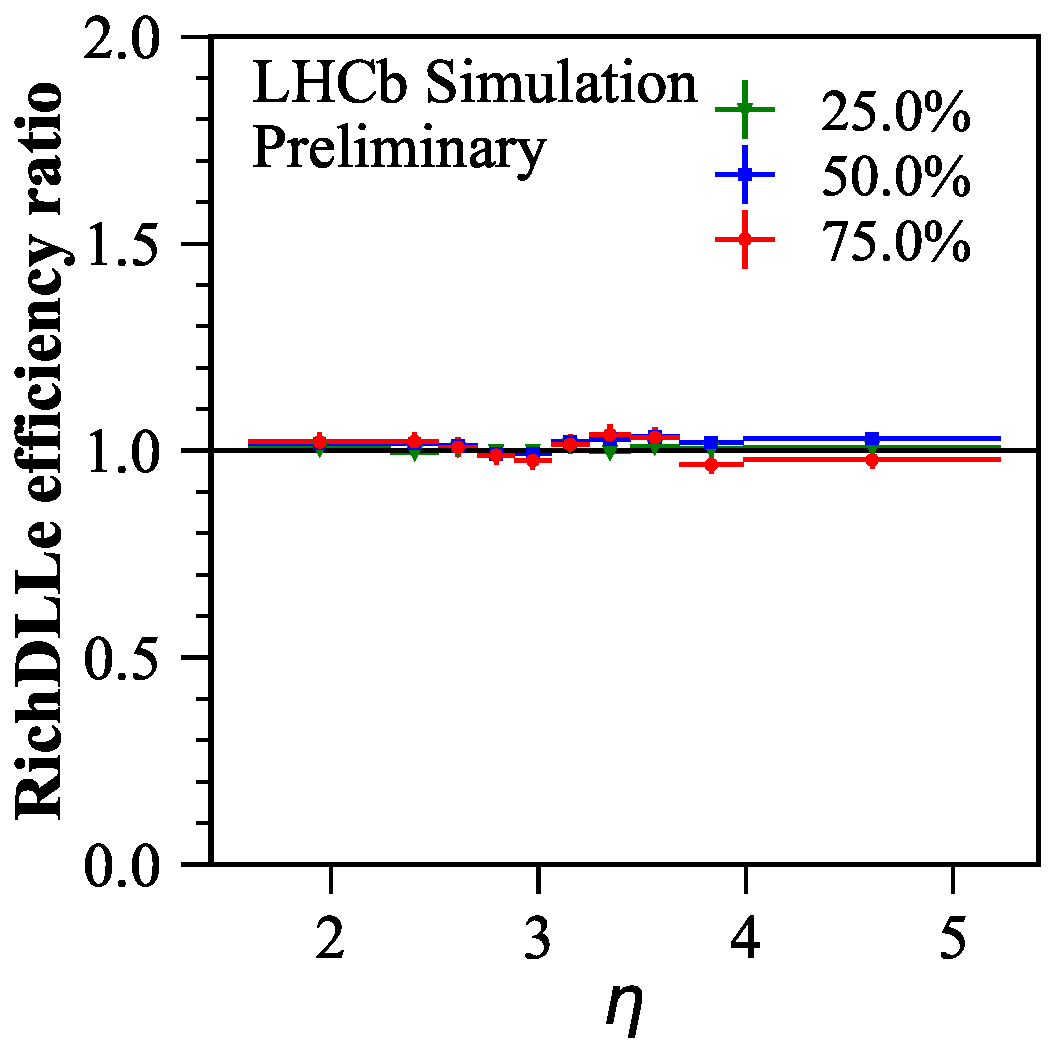
\includegraphics[width=0.3\linewidth]{eff_ratio_RichDLLe_vs_Brunel_ETA_at_[0.05, 0.1, 0.25, 0.5, 0.75, 0.9, 0.95].pdf} &
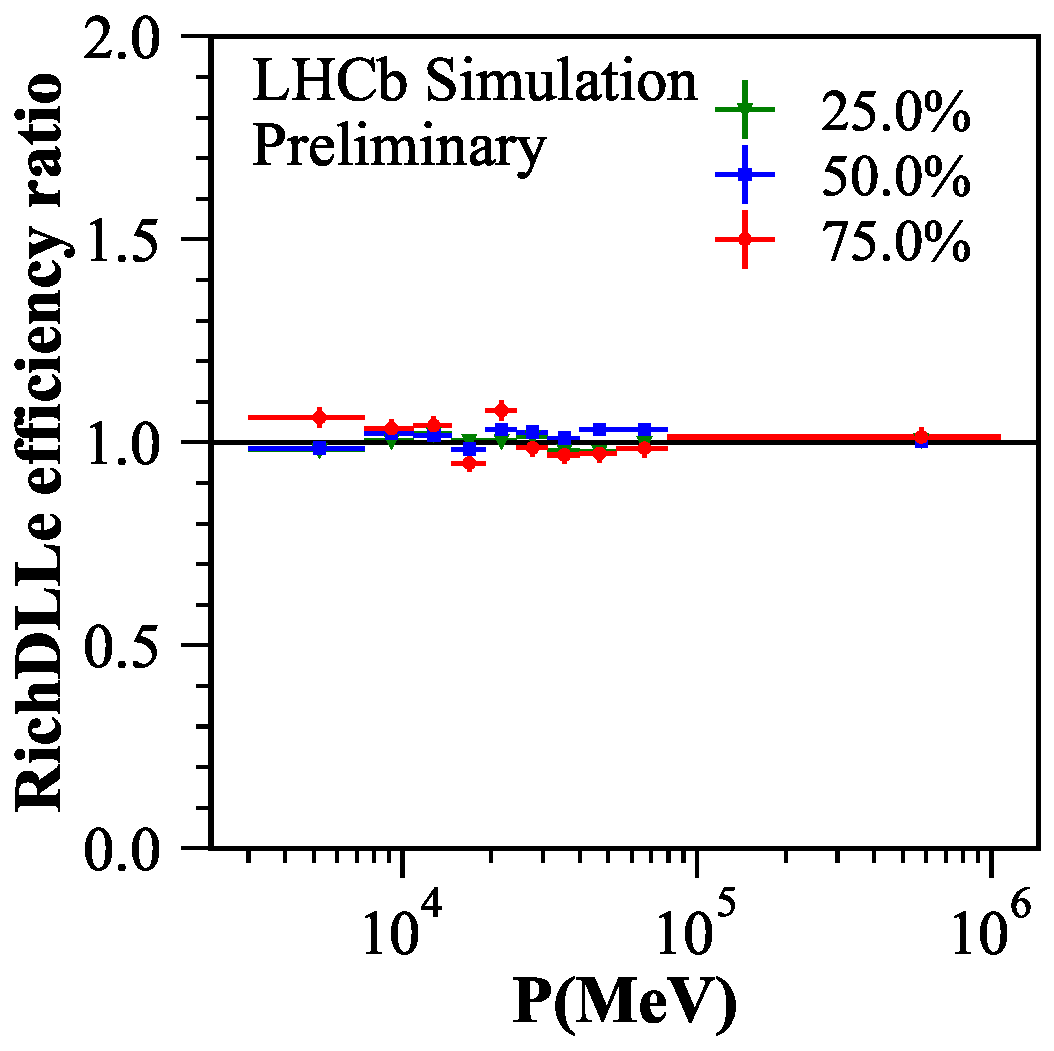
\includegraphics[width=0.3\linewidth]{eff_ratio_RichDLLe_vs_Brunel_P_at_[0.05, 0.1, 0.25, 0.5, 0.75, 0.9, 0.95].pdf} &
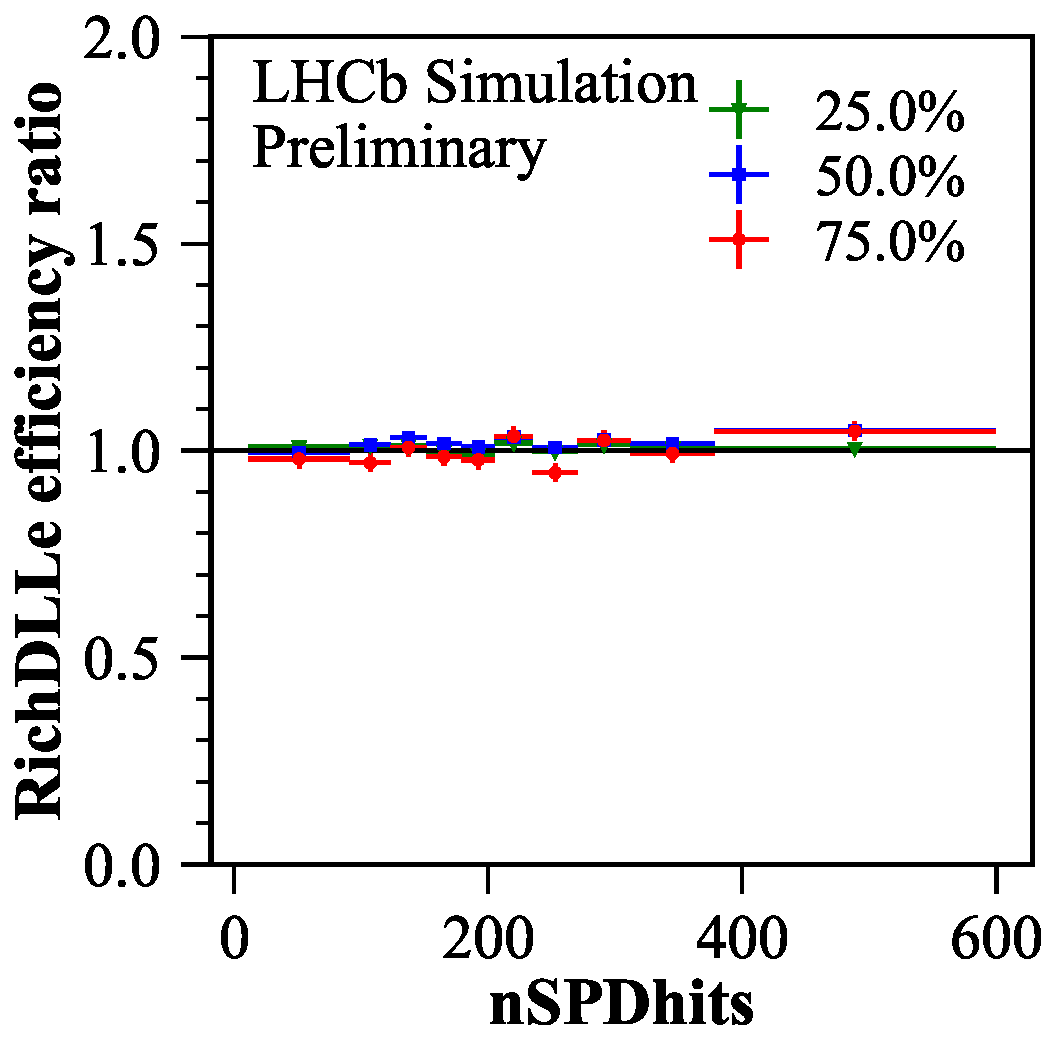
\includegraphics[width=0.3\linewidth]{eff_ratio_RichDLLe_vs_nSPDhits_at_[0.05, 0.1, 0.25, 0.5, 0.75, 0.9, 0.95].pdf} \\
\vspace{-0.2cm}

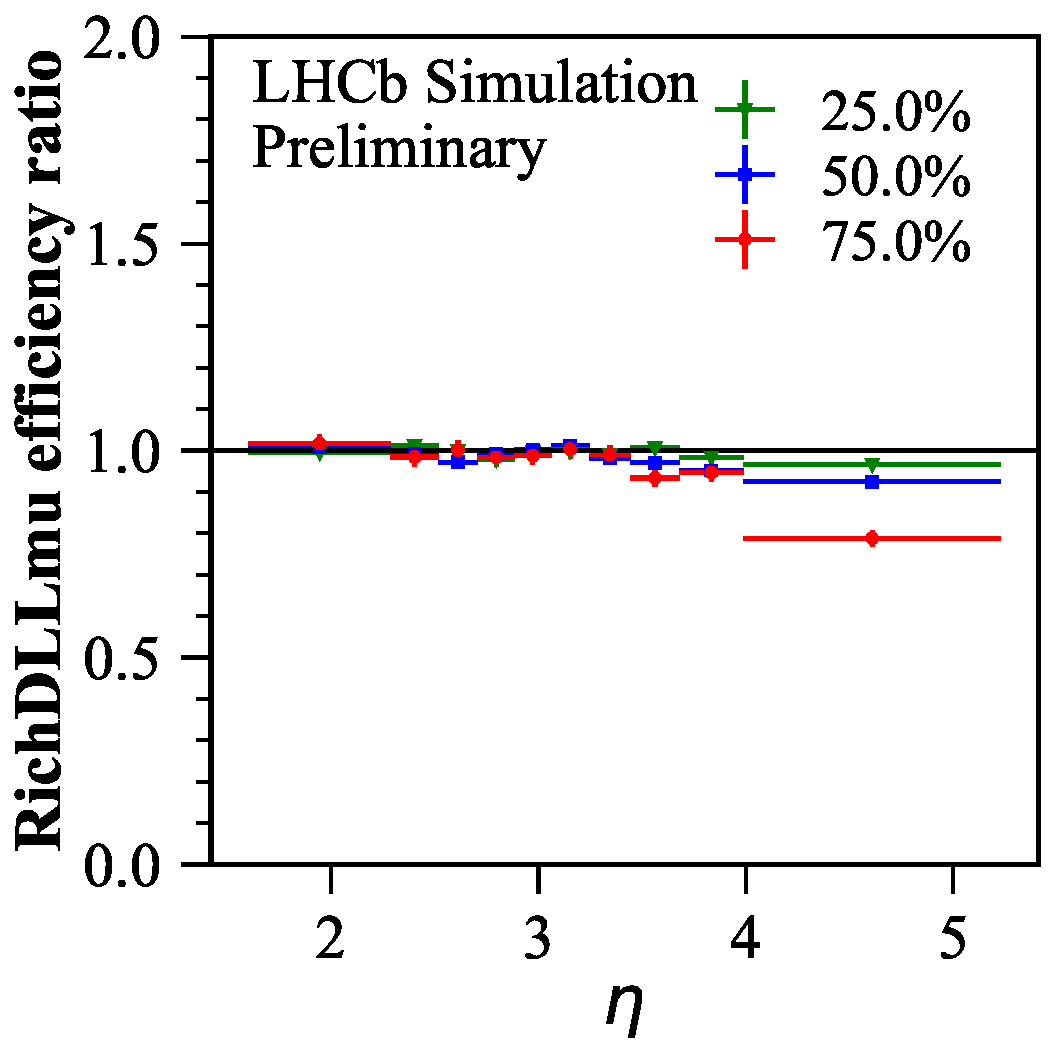
\includegraphics[width=0.32\linewidth]{eff_ratio_RichDLLmu_vs_Brunel_ETA_at_[0.05, 0.1, 0.25, 0.5, 0.75, 0.9, 0.95].pdf} &
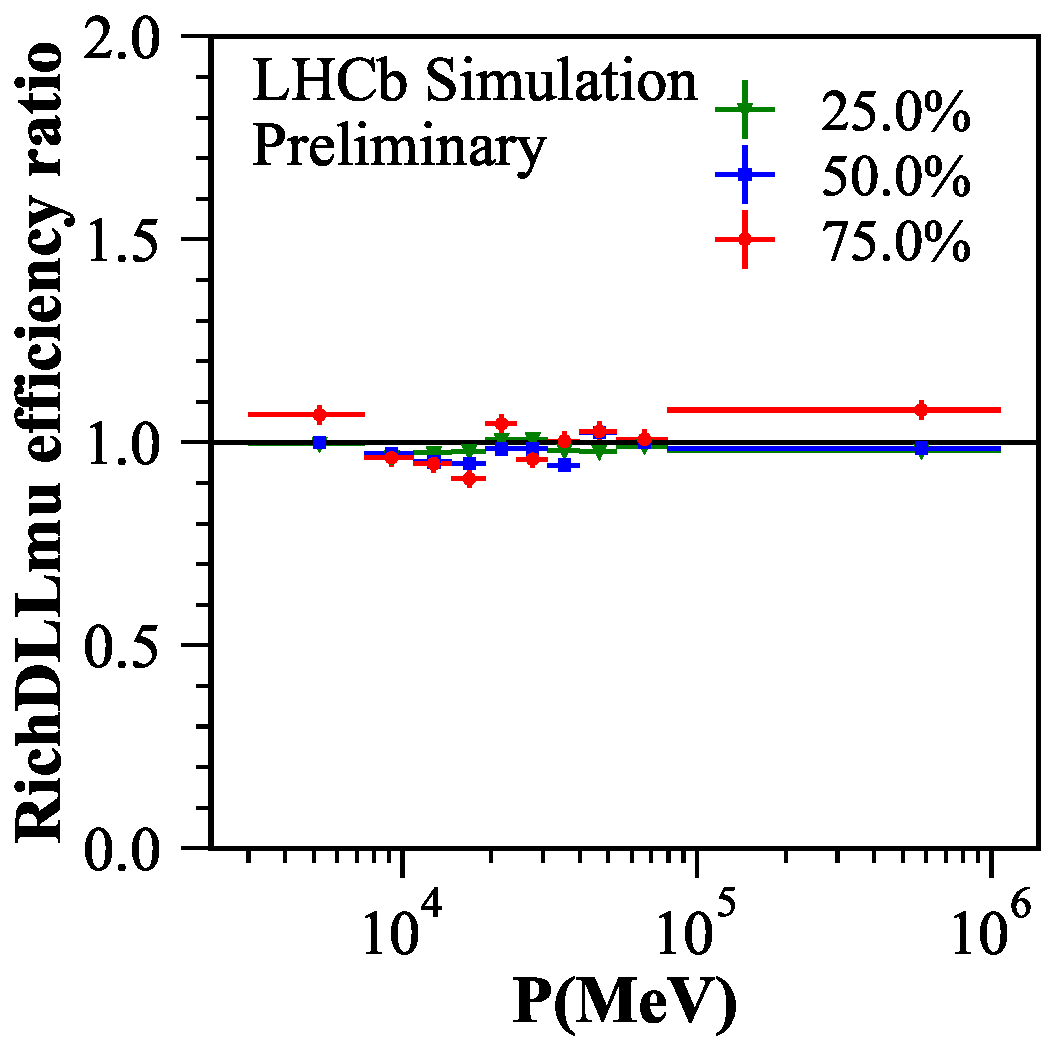
\includegraphics[width=0.32\linewidth]{eff_ratio_RichDLLmu_vs_Brunel_P_at_[0.05, 0.1, 0.25, 0.5, 0.75, 0.9, 0.95].pdf} &
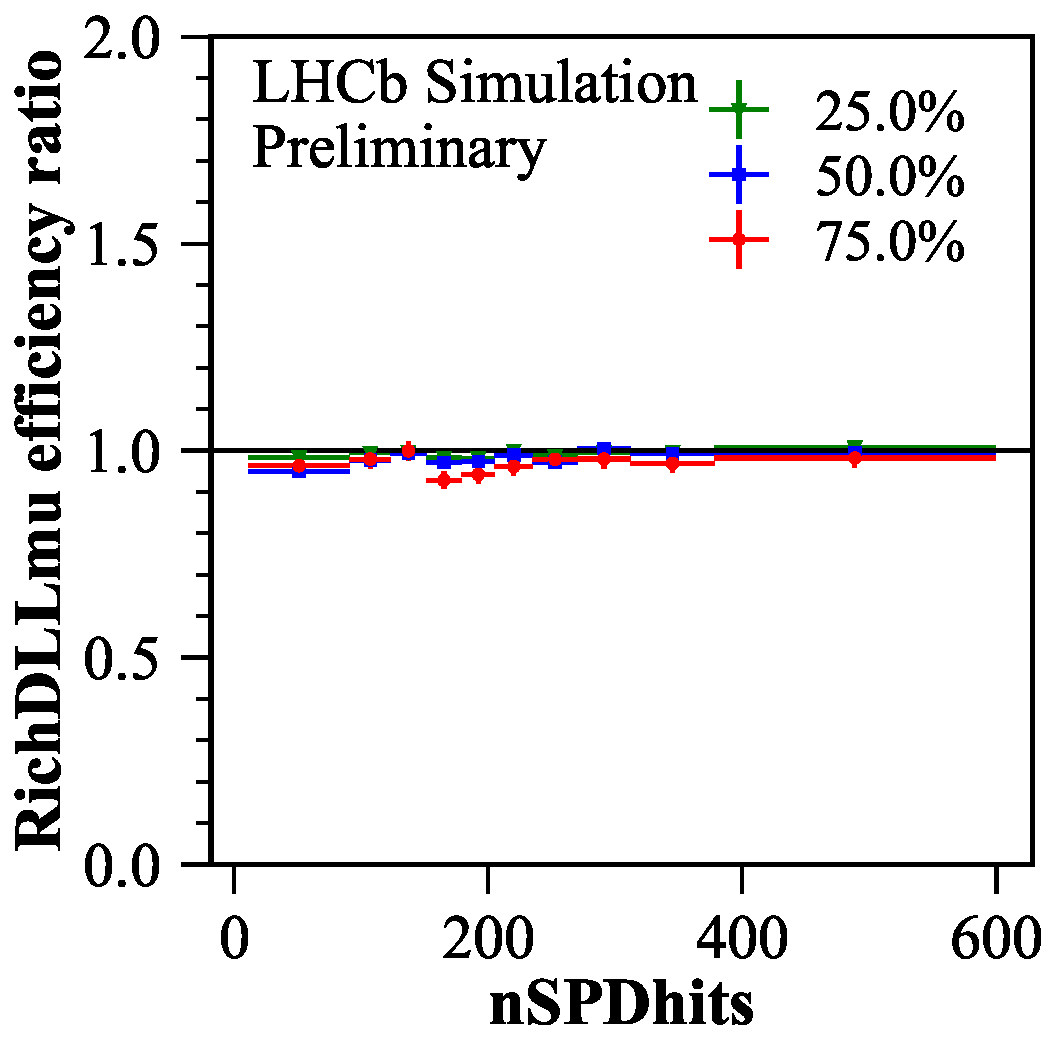
\includegraphics[width=0.32\linewidth]{eff_ratio_RichDLLmu_vs_nSPDhits_at_[0.05, 0.1, 0.25, 0.5, 0.75, 0.9, 0.95].pdf} \\
\vspace{-0.2cm}
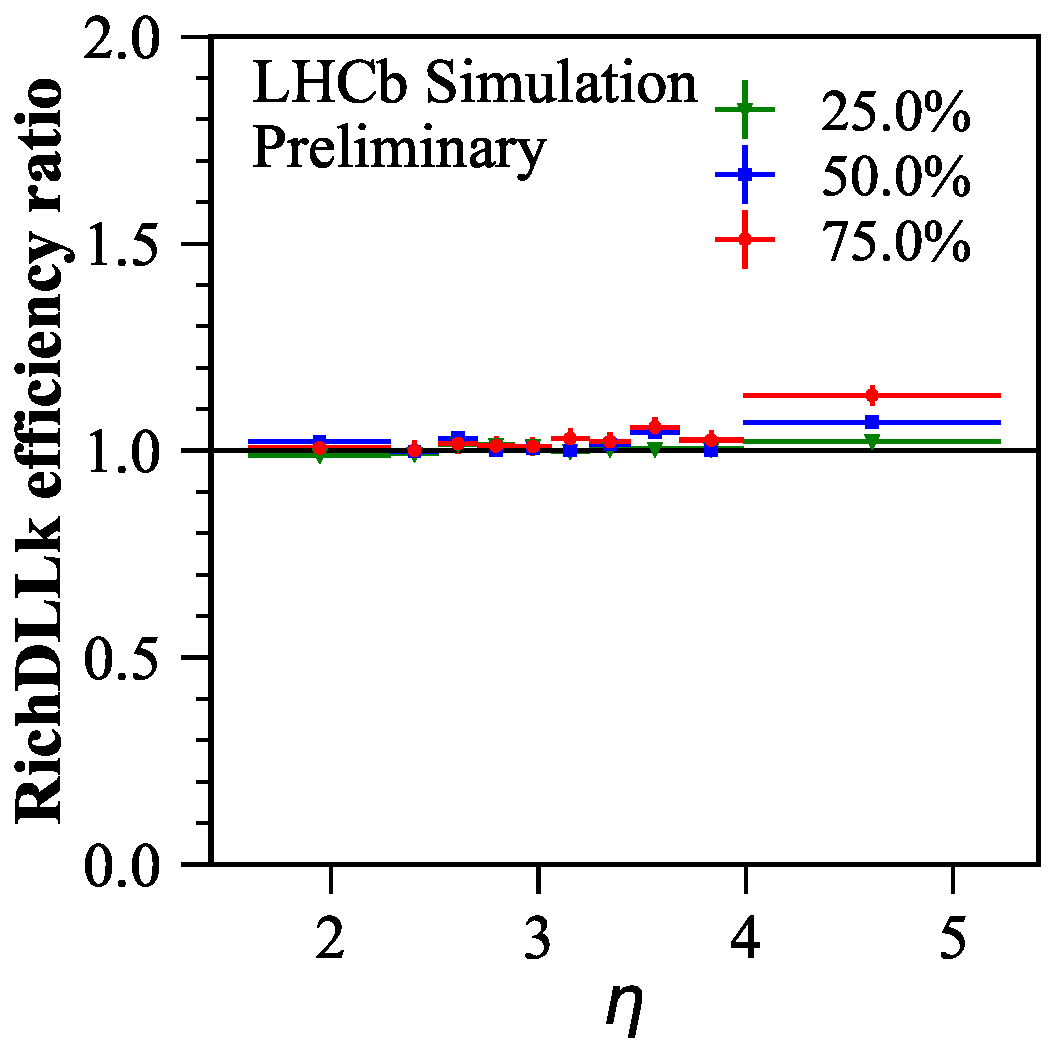
\includegraphics[width=0.32\linewidth]{eff_ratio_RichDLLk_vs_Brunel_ETA_at_[0.05, 0.1, 0.25, 0.5, 0.75, 0.9, 0.95].pdf} &
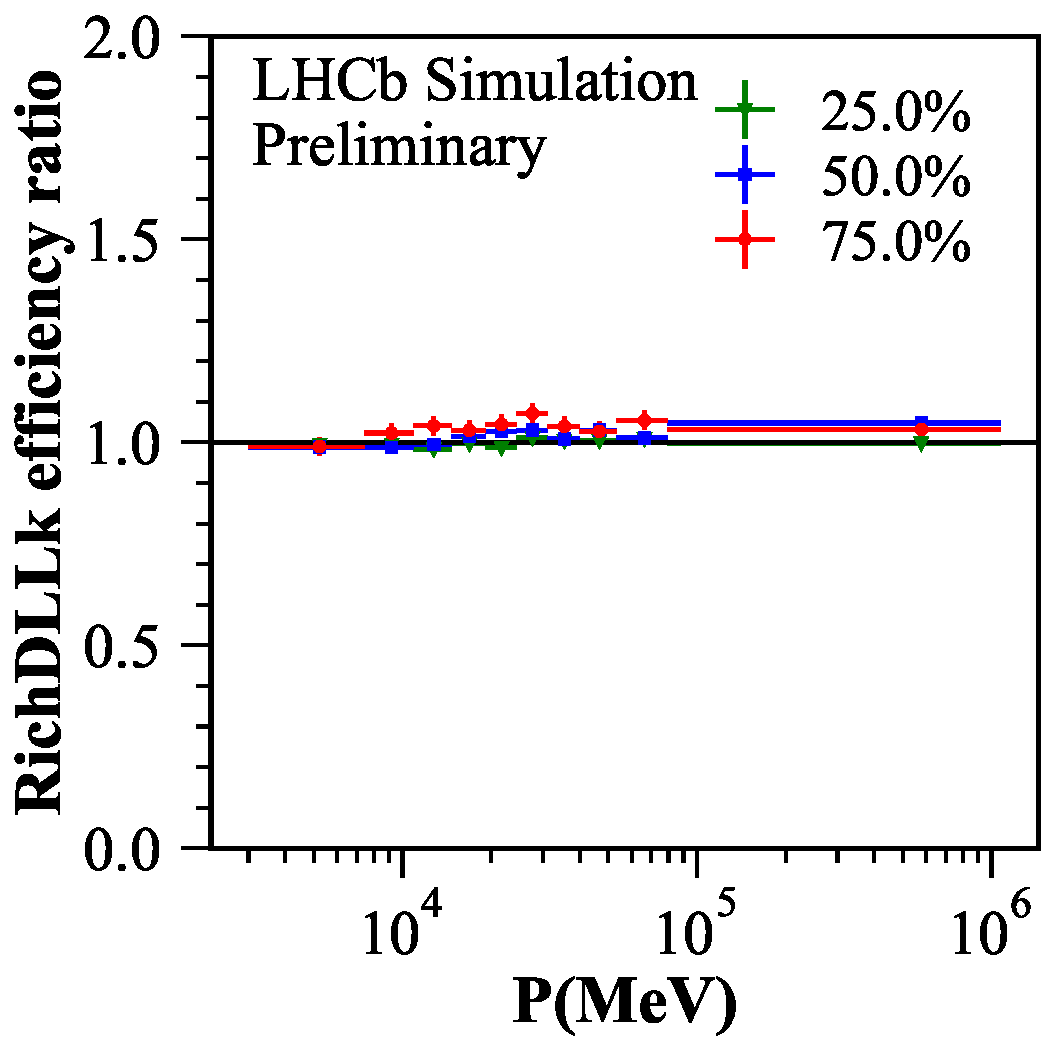
\includegraphics[width=0.32\linewidth]{eff_ratio_RichDLLk_vs_Brunel_P_at_[0.05, 0.1, 0.25, 0.5, 0.75, 0.9, 0.95].pdf} &
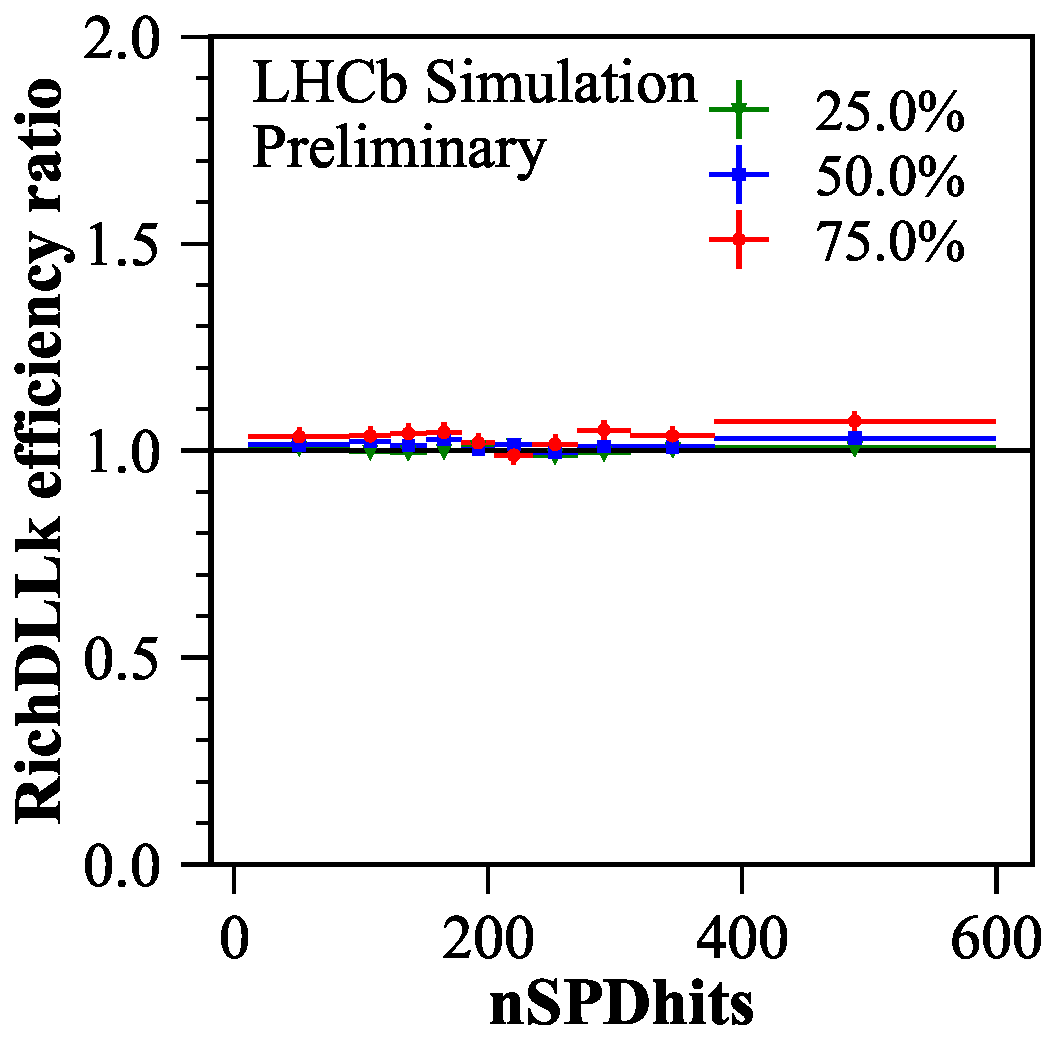
\includegraphics[width=0.32\linewidth]{eff_ratio_RichDLLk_vs_nSPDhits_at_[0.05, 0.1, 0.25, 0.5, 0.75, 0.9, 0.95].pdf} \\
\vspace{-0.2cm}
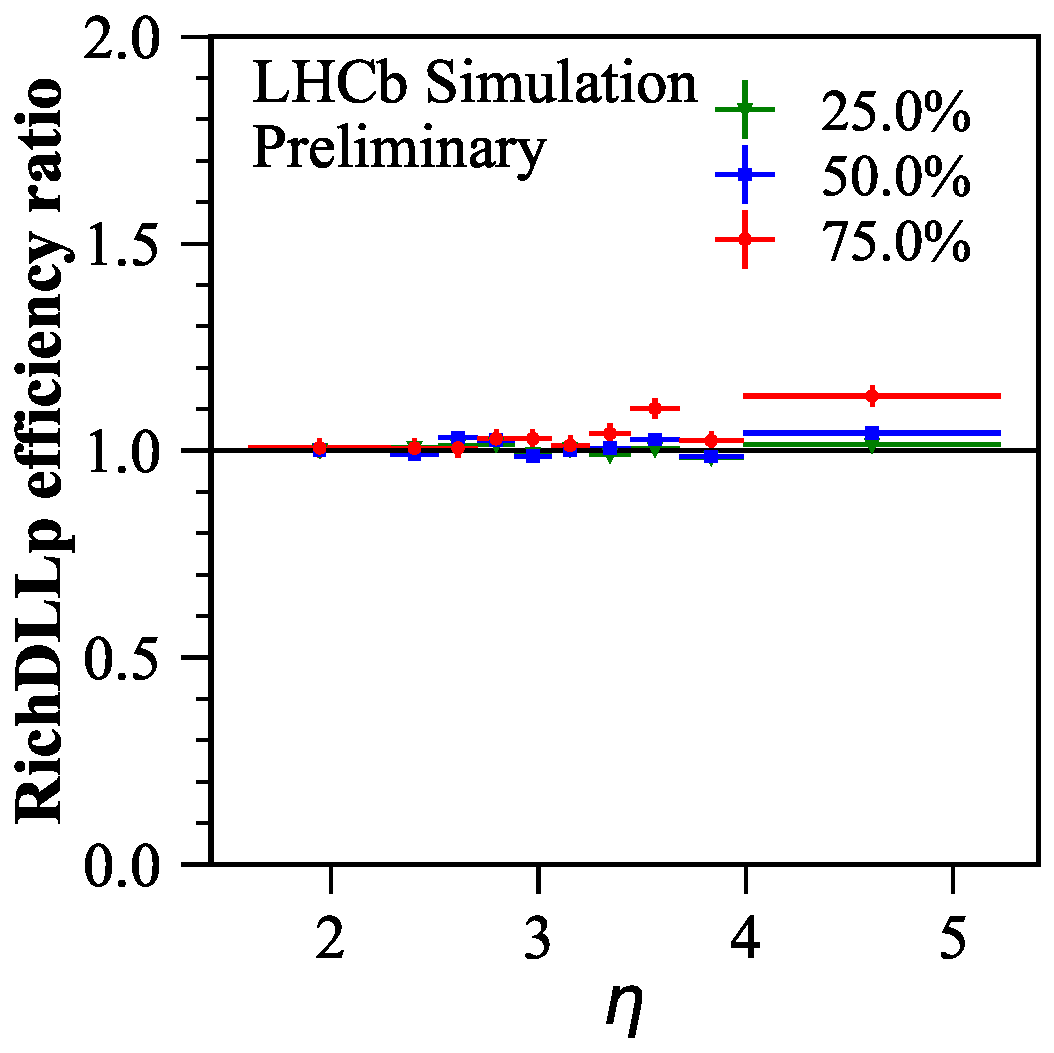
\includegraphics[width=0.32\linewidth]{eff_ratio_RichDLLp_vs_Brunel_ETA_at_[0.05, 0.1, 0.25, 0.5, 0.75, 0.9, 0.95].pdf} &
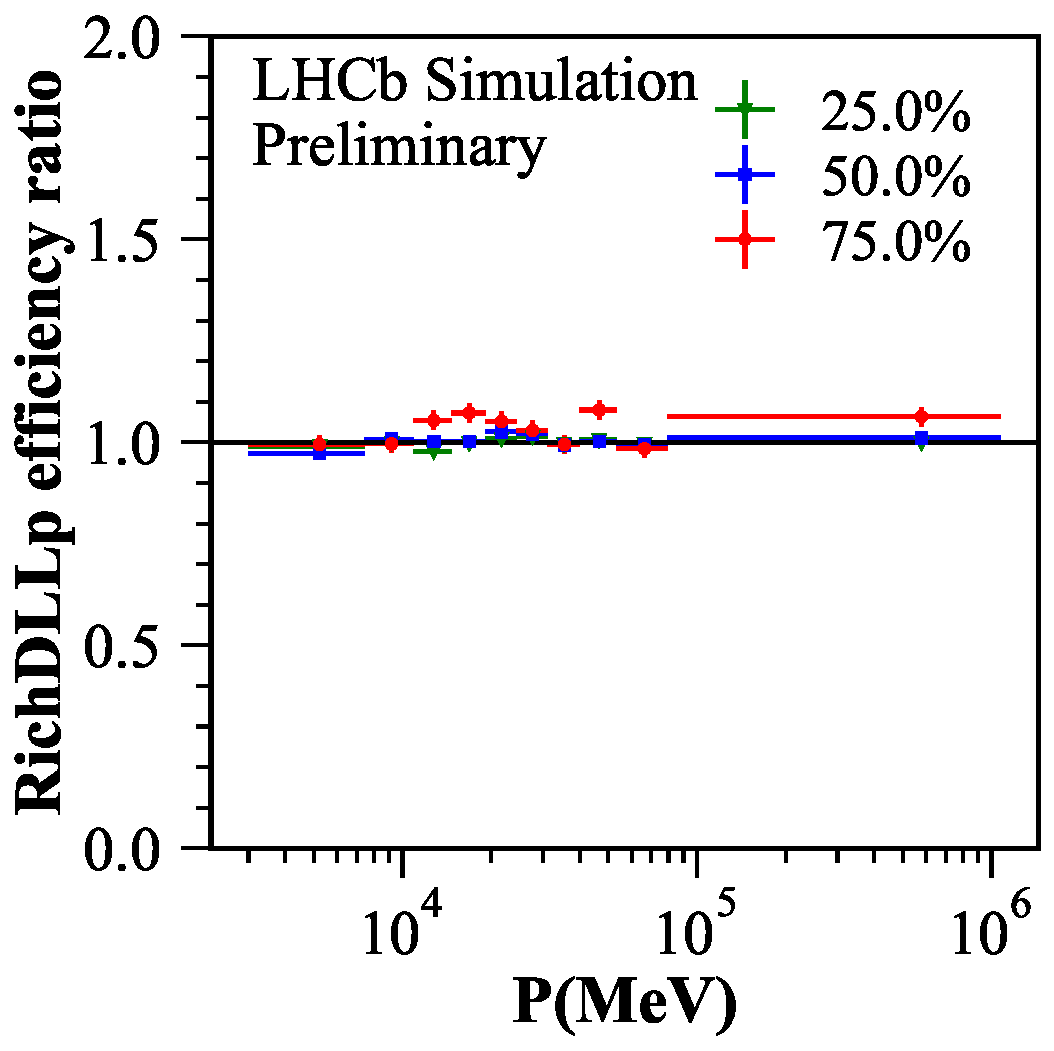
\includegraphics[width=0.32\linewidth]{eff_ratio_RichDLLp_vs_Brunel_P_at_[0.05, 0.1, 0.25, 0.5, 0.75, 0.9, 0.95].pdf} &
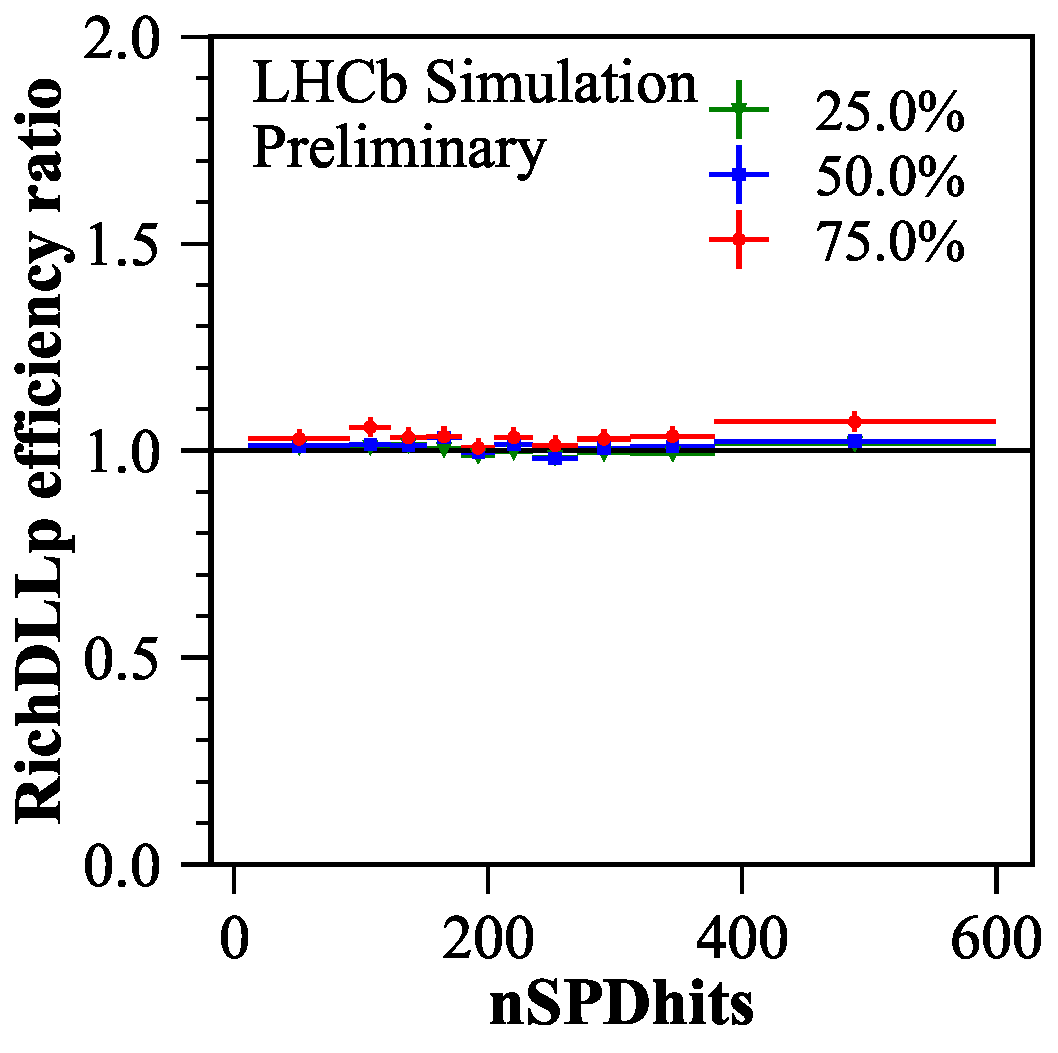
\includegraphics[width=0.32\linewidth]{eff_ratio_RichDLLp_vs_nSPDhits_at_[0.05, 0.1, 0.25, 0.5, 0.75, 0.9, 0.95].pdf} \\
\vspace{-0.2cm}
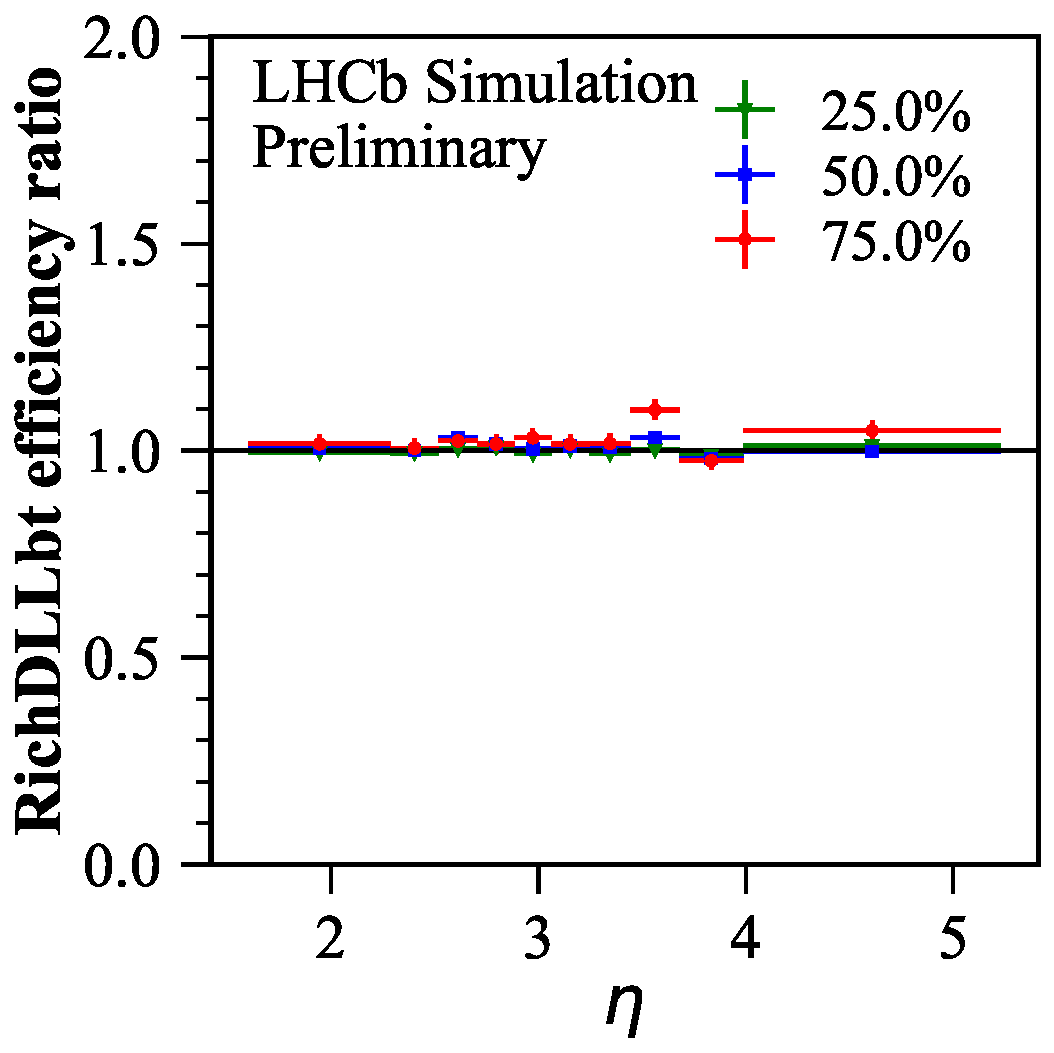
\includegraphics[width=0.32\linewidth]{eff_ratio_RichDLLbt_vs_Brunel_ETA_at_[0.05, 0.1, 0.25, 0.5, 0.75, 0.9, 0.95].pdf} &
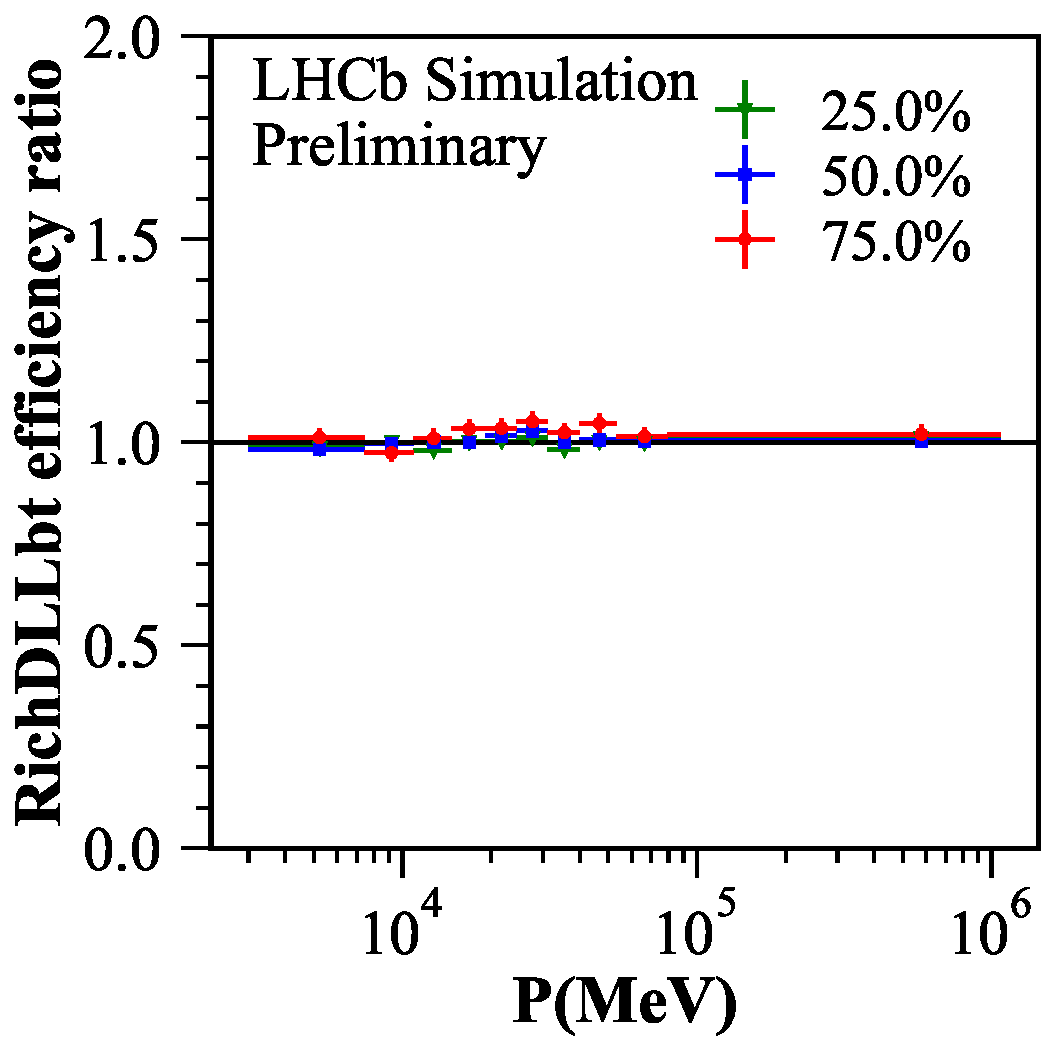
\includegraphics[width=0.32\linewidth]{eff_ratio_RichDLLbt_vs_Brunel_P_at_[0.05, 0.1, 0.25, 0.5, 0.75, 0.9, 0.95].pdf} &
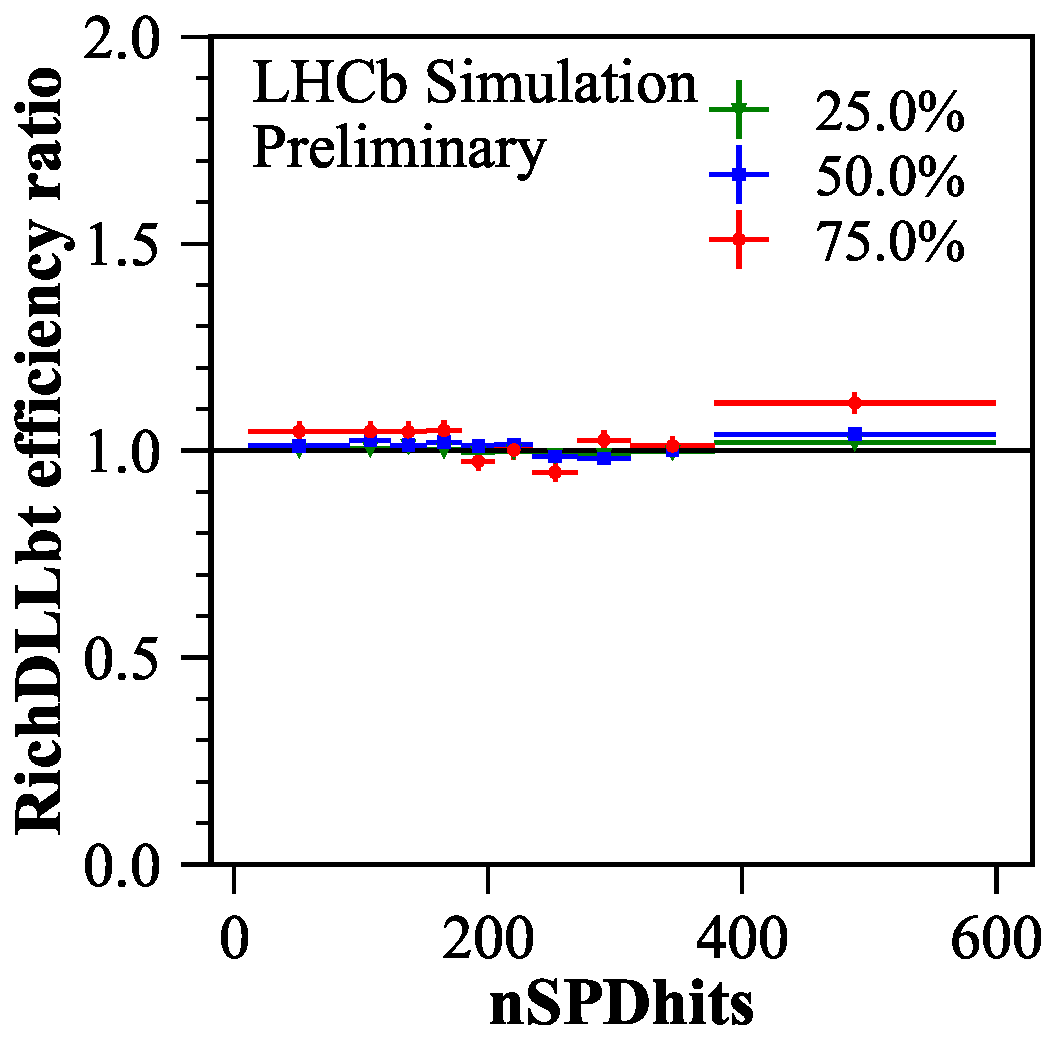
\includegraphics[width=0.32\linewidth]{eff_ratio_RichDLLbt_vs_nSPDhits_at_[0.05, 0.1, 0.25, 0.5, 0.75, 0.9, 0.95].pdf} \\
\vspace{-0.2cm}
\end{tabular}

\end{document}

